\section{Элементы функциональной схемы}
\label{s::ch::practice::elements}

В данном разделе приводится необходимый минимум сведений для изображения и понимания функциональных схем. За исчерпывающей информацией обращайтесь к стандарту \cite{bib:gost:fs}.


\subsection{Сигналы, шины, жгуты}


Отдельная \emph{сигнальная линия} соответствует проводнику (проводу), который передает логические значения 0 или 1. Сигнальная линия на схеме изображается тонкой линией, соедняющей выход некоторого элемента со входом некоторого элемента. 

Множество внешних (интерфейсных) сигнальных линий принято объединять в \emph{шины}. Шина на схеме изображается толстой линией и обязательно именуется: сверху над линией в удобном месте подписывается имя шины (на рисунке \ref{fig::ch::practice::bus} изображена шина $X$). В общем случае шин на схеме может быть несколько. В качестве имени шины обычно выбирают заглавную литеру: $X$, $Y$, $Z$, $P$, а если шины разделены по функциональному назначению, то они могут быть названы: ШД --- шина данных, ША --- шина адреса, ШУ --- шина управления и т.д.

\begin{figure}[!ht]
    \centering
    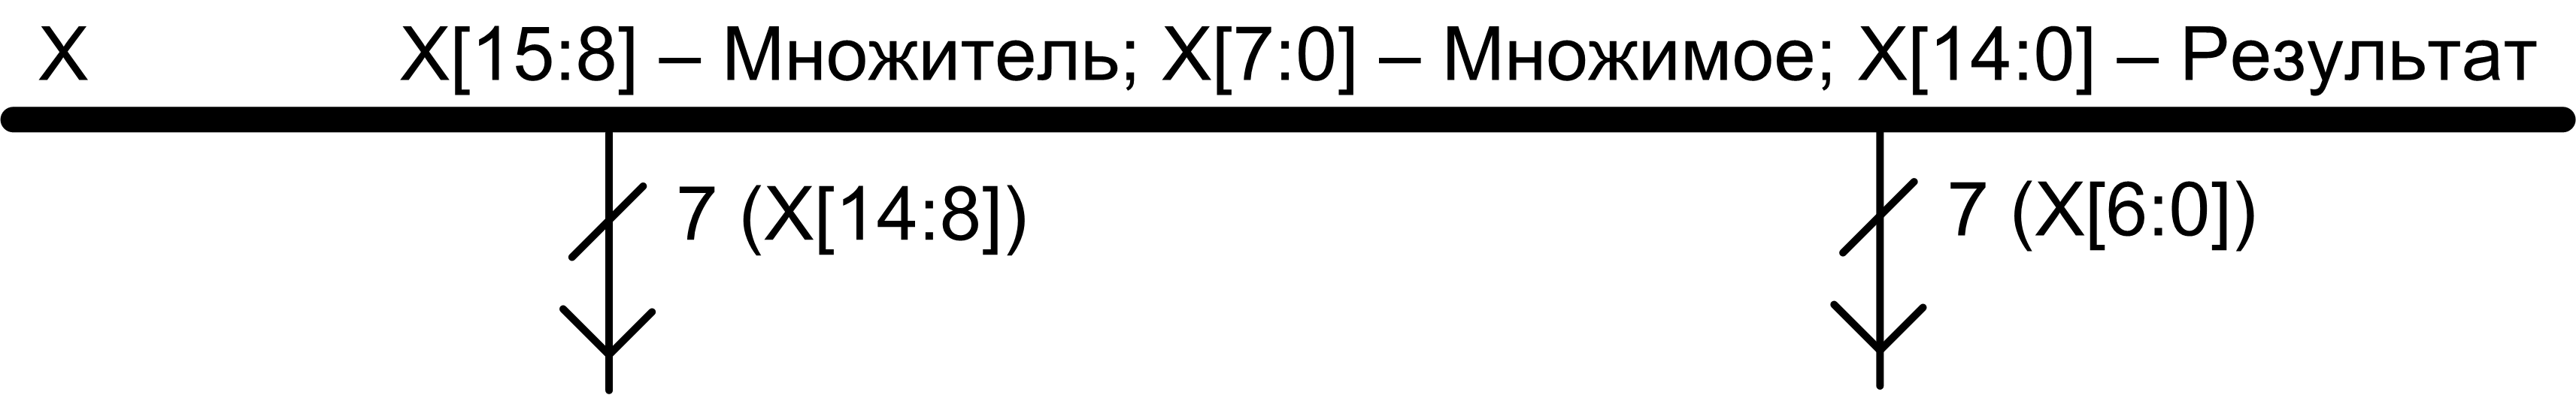
\includegraphics{fig/bus}
    \caption{Изображение шин и жгутов}
    \label{fig::ch::practice::bus}
\end{figure}

Чтобы не рисовать множество параллельных сигнальных линий, в случае, когда передается группа бит, на схеме изображают \emph{жгут}. Жгут также изображается тонкой линией, на которой в произвольном месте (но не на концах) тонкими линиями рисуется тупоугольная стрелка, указвающая направление передачи, сверху от стрелки жгут перечеркивается косой чертой и справа указывается разрядность жгута. В случае когда требуется указать, какие разряды шины отведены в жгут, в скобках после разрядности перечисляются обозначения групп сигнальных линий в составе шины. На рисунке \ref{fig::ch::practice::bus} от шины $X$ отведены два жгута по $7$ разрядов каждый.

\emph{Сигналы} разделяют на осведомительные и управляющие. Управляющие сигналы обычно обозначаются: $Y0$, $Y1$, $Y2$,\ldots, а осведомительные --- $P0$, $P1$, $P2$,\ldots Если управляющий сигнал подается на вход элемента, а не на управление, то стрелку не рисуют.  На рисунке \ref{fig::ch::practice::controls} изображен $8$-и разрядный регистр (подробнее о регистрах см. раздел \ref{sss::ch::practice::regiter}), который управляется сигналами $Y0$, $Y1$. Седьмой разряд выхода регистра используется как осведомительный сигнал $P0$. На входные разряды с $0$ по $3$ подаются соответственно сигналы с $3$ по $6$ шины $X$. На вход $RG1[7:4]$ подается двоичное значение $(0011)_2$.

Управляющие сигналы подводятся стрелками, входящими в управляемый блок справа. Осведомительные отводятся с выходов стрелкой, направленной вниз или влево.

\begin{figure}[!ht]
    \centering
    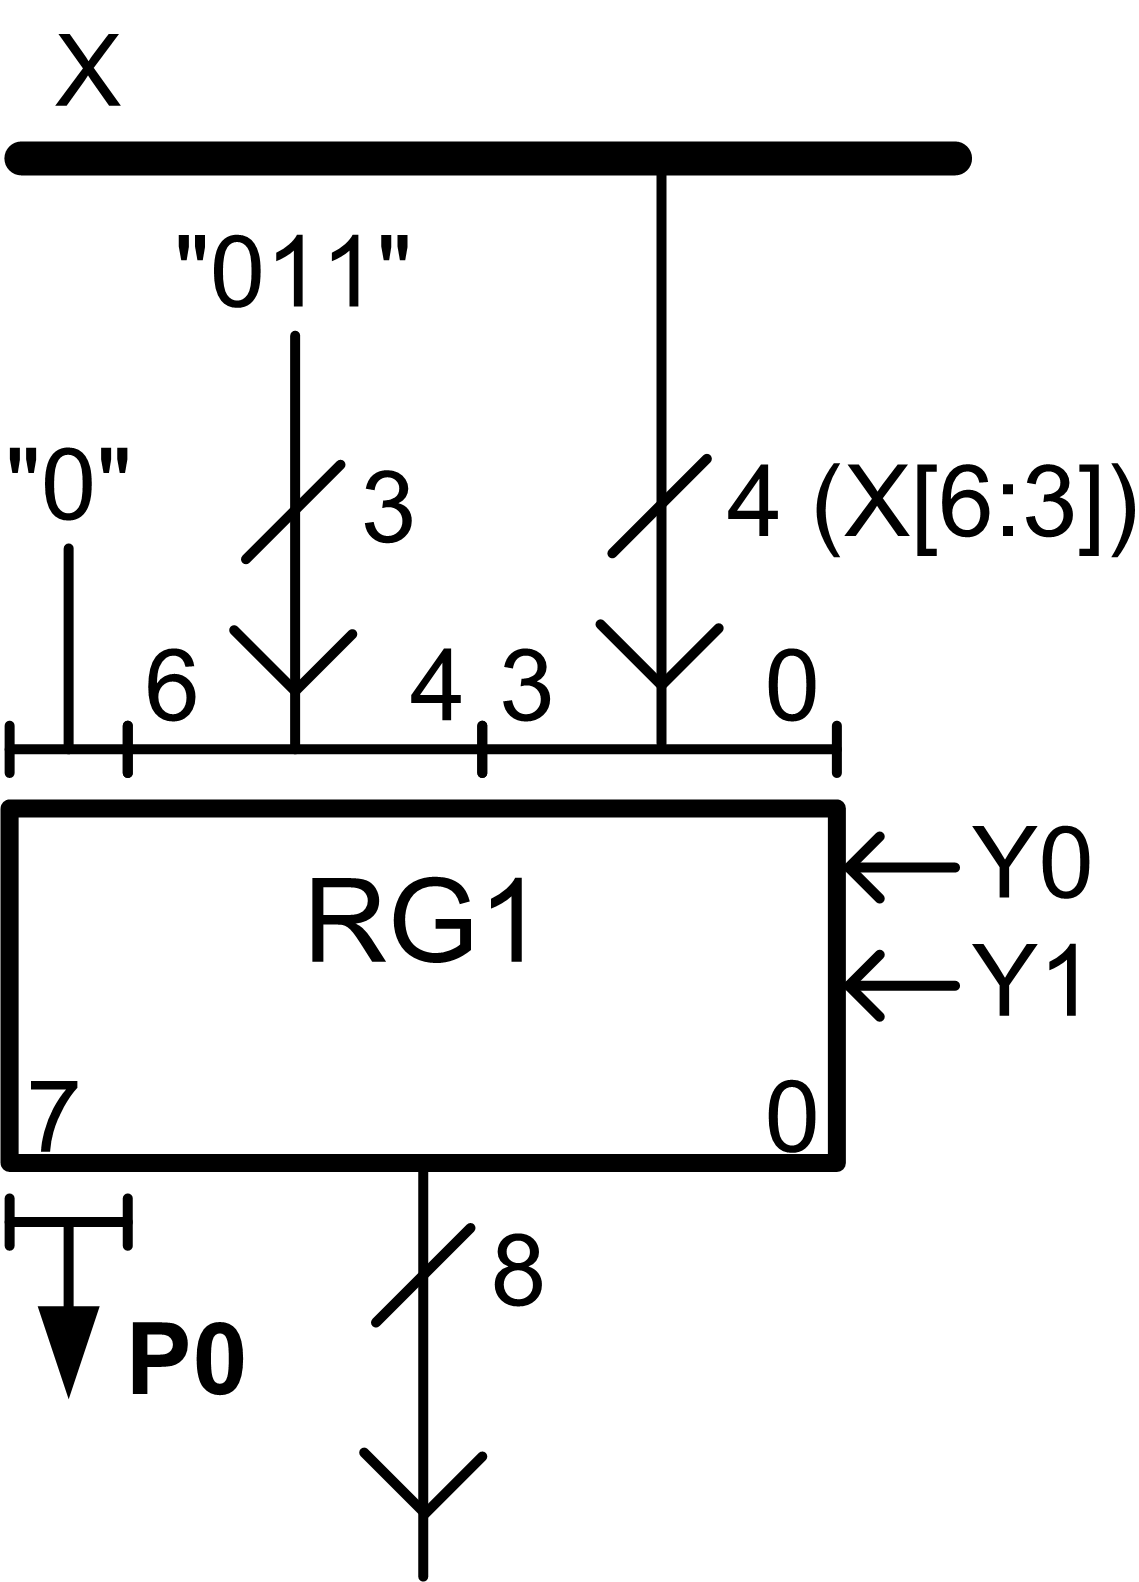
\includegraphics{fig/controls}
    \caption{Входы, выходы и управляющие сигналы регистра}
    \label{fig::ch::practice::controls}
\end{figure}

\begin{figure}[!ht]
    \centering
    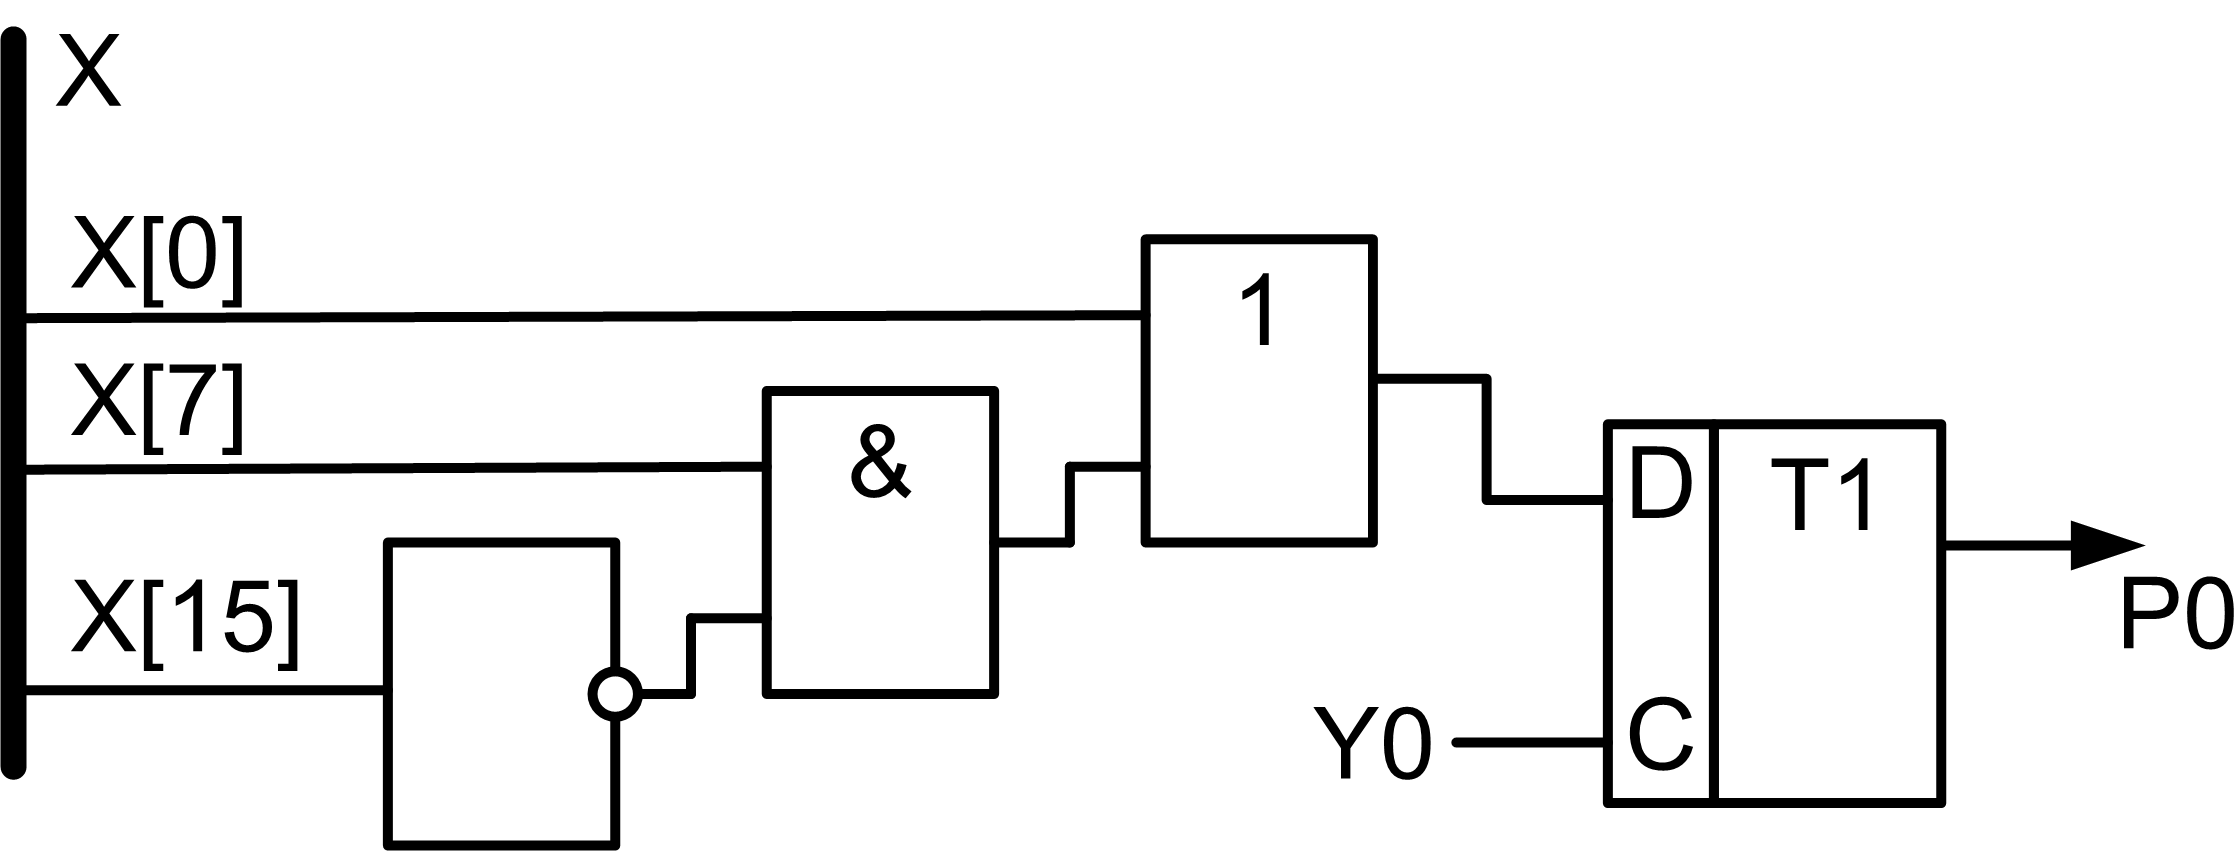
\includegraphics{fig/logic}
    \caption{Логическая схема}
    \label{fig::ch::practice::logic}
\end{figure}

Входы большинства элементов на схеме подводятся сверху, а выходы --- снизу. Исключением являются элементы логической схемы и триггеры (см. рисунок \ref{fig::ch::practice::logic}), в которой входы подаются слева, а выходы снимаются справа. В любом случае недопустимо разворачивать или переворачивать блоки.

Если о разрядности входов можно судить по разрядности выходов, то допустимо подписывать только разрядности выходов элементов.


\subsection{Элементы логики}

Элементы логики отличаются от элементов памяти тем, что представляют собой реализацию однотактной функции: выход формируется за один такт времени и зависит только от информации на входах. У элементов логики нет внутреннего состояния. Типичные элементы логики это: логические схемы (И, ИЛИ, НЕ, XOR, И-НЕ, и т.д.), мультиплексоры, сумматоры, шинные формирователи и т.д.


\subsubsection{Многовходовые логические функции}

На схемах элементы, реализующие многовходовую ассоциативную и комутативную логическую функцию (И, ИЛИ, XOR), допустимо изображать одним элементом, как на рисунке \ref{fig::ch::practice::bigLogic}.
\begin{figure}[!ht]
    \centering
    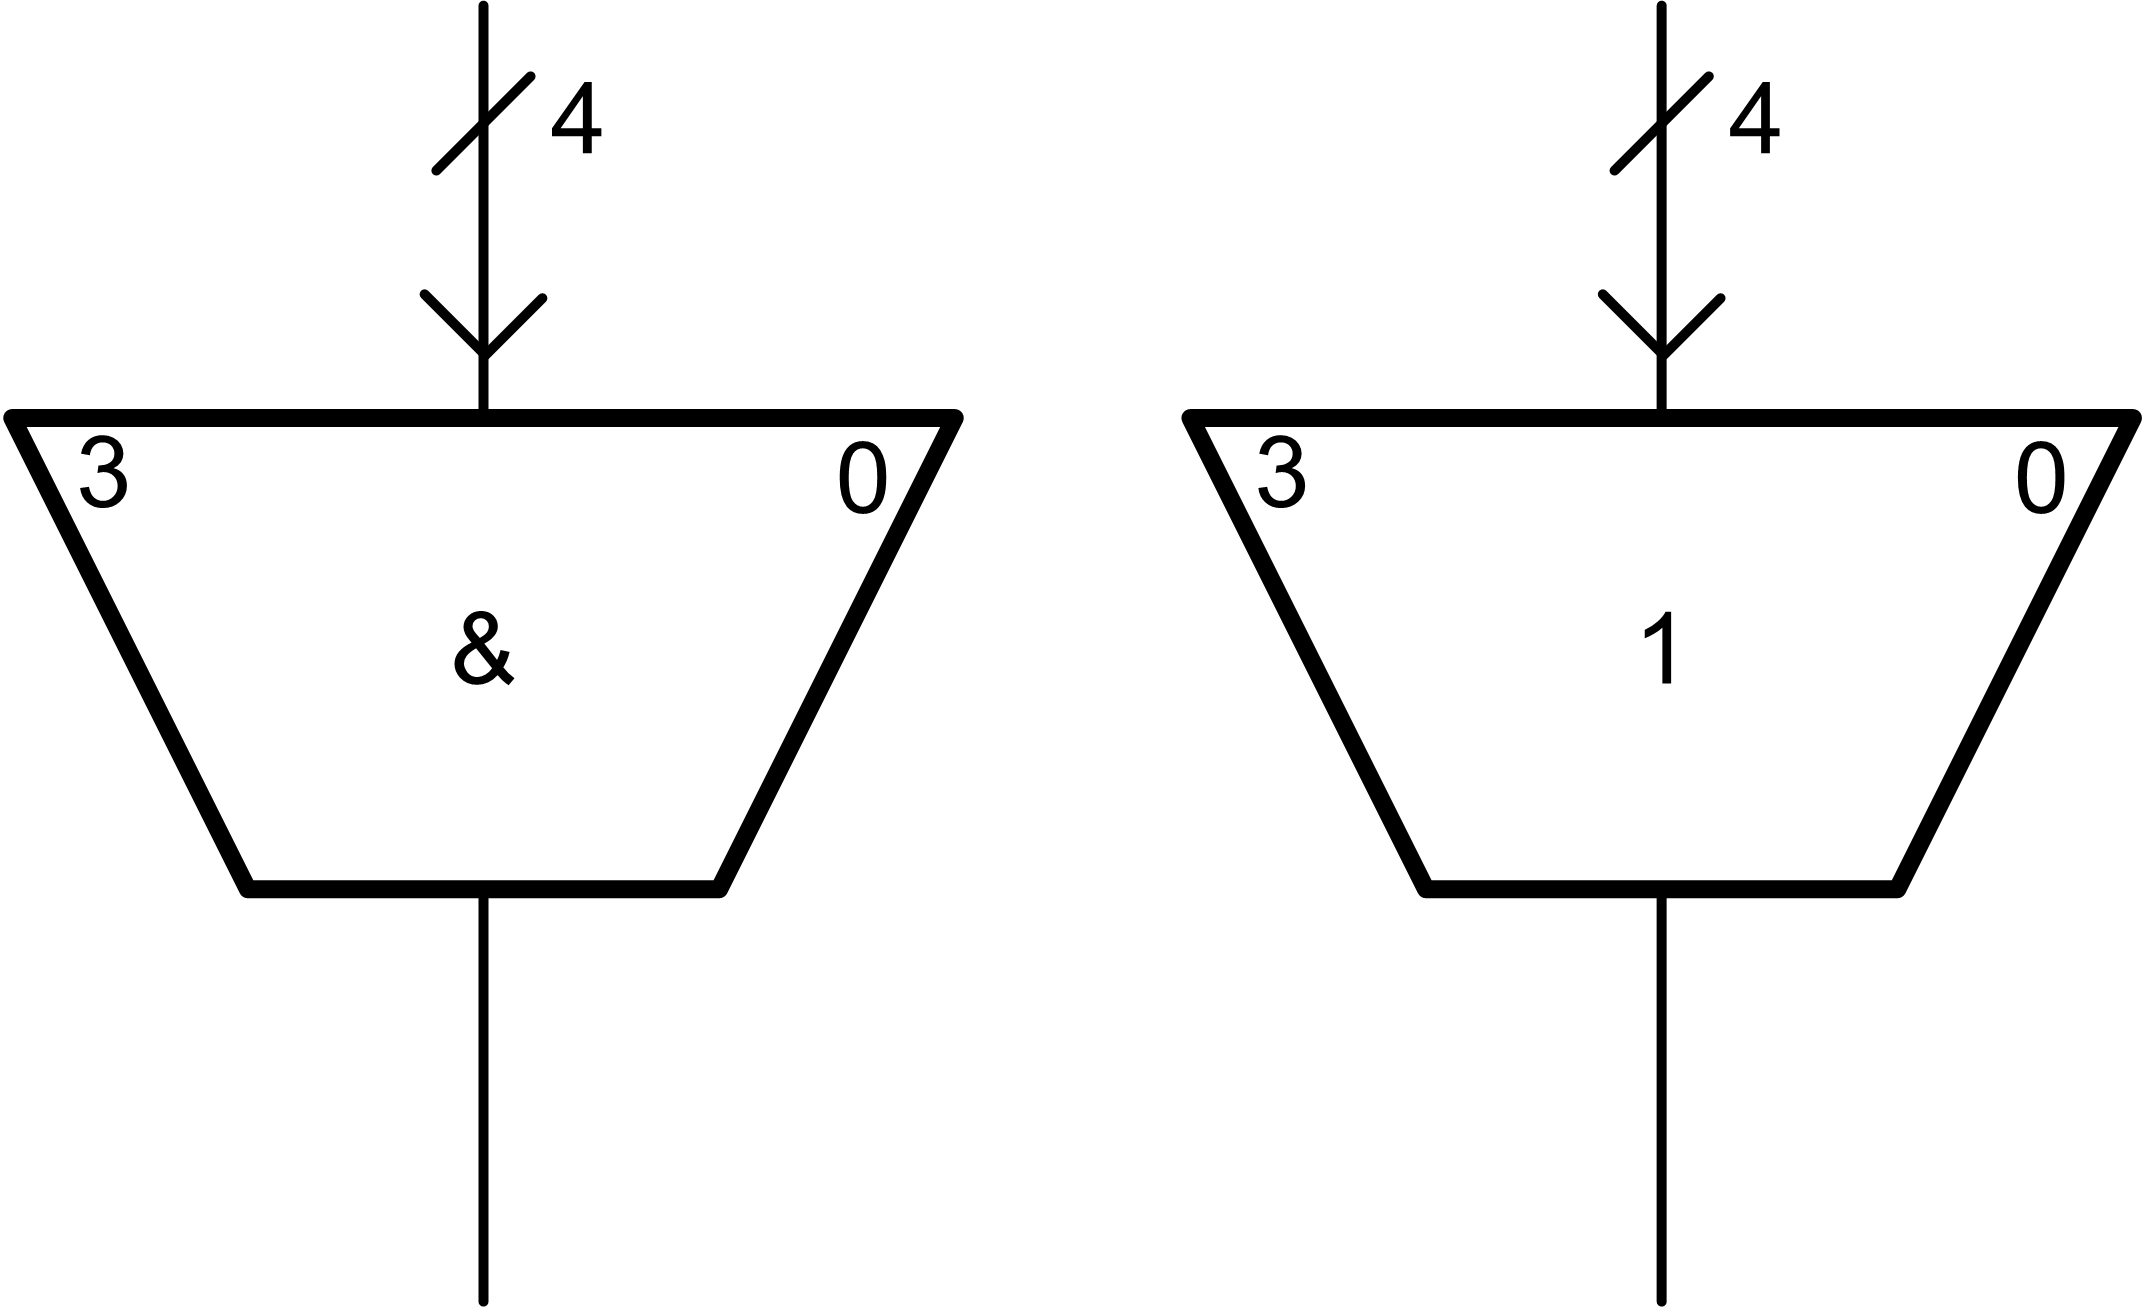
\includegraphics{fig/bigLogic}
    \caption{$4$-х входовые функции И, ИЛИ}
    \label{fig::ch::practice::bigLogic}
\end{figure}

Выход такого элемента --- одноразрядный.


\subsubsection{Инвертор}

На схемах многоразрядный инвертор изображается как рисунке \ref{fig::ch::practice::invertor}.
\begin{figure}[!ht]
    \centering
    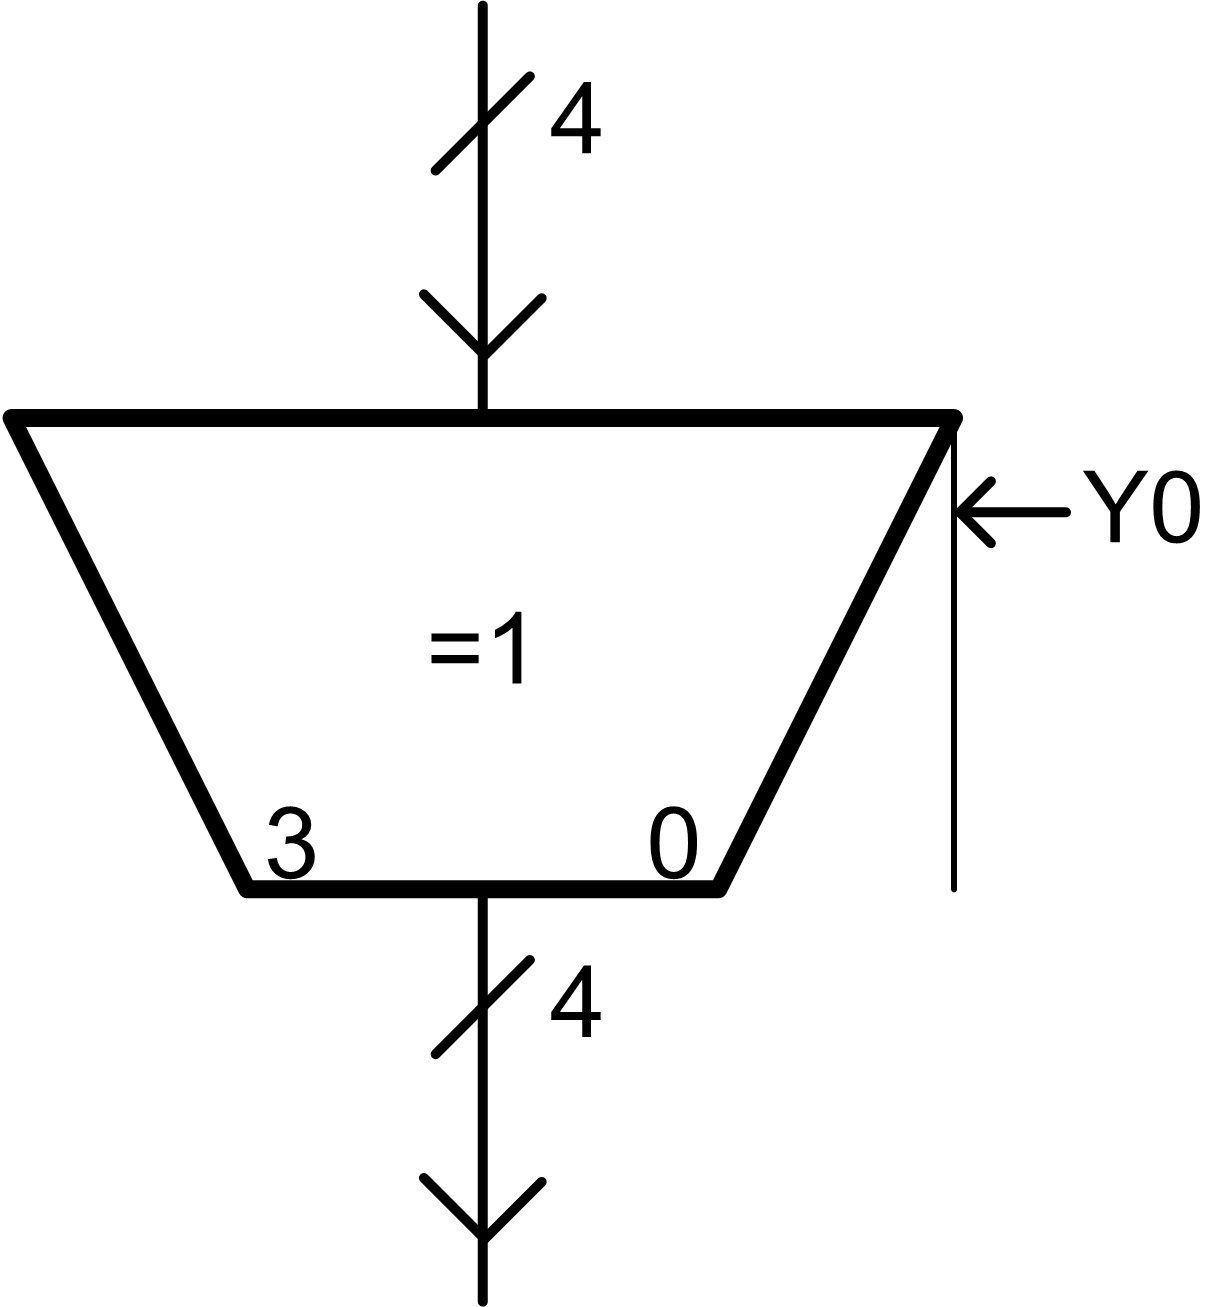
\includegraphics{fig/invertor}
    \caption{$4$-х разрядный инвертор}
    \label{fig::ch::practice::invertor}
\end{figure}

Если значение единственного управляющего сигнала 0, то разряды входа без изменений подаются на выход, иначе на выходе формируется поразрядная инверсия входа.

\subsubsection{Мультиплексор}

Условное графическое обозначение мультиплексора приведено на рисунке \ref{fig::ch::practice::mux}.
\begin{figure}[!ht]
    \centering
    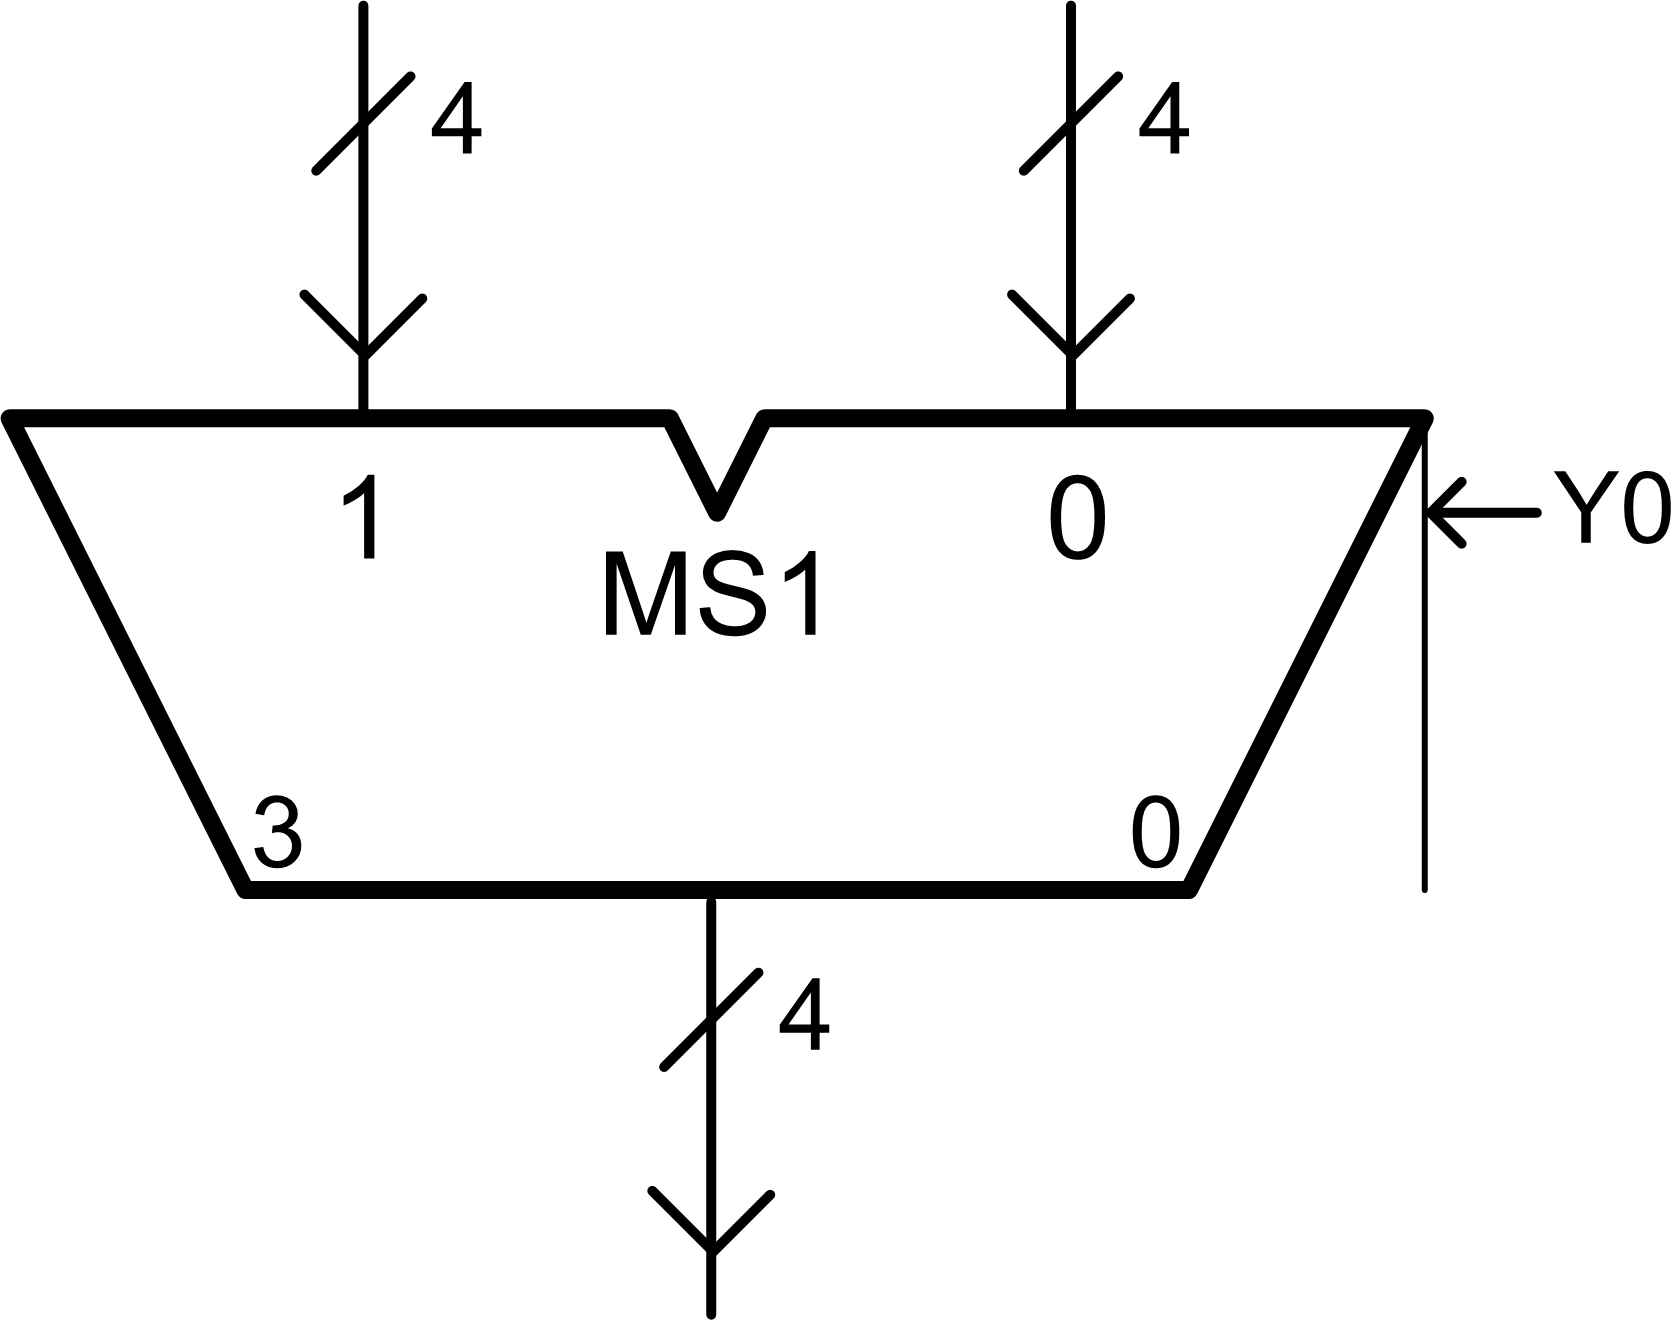
\includegraphics{fig/mux}
    \caption{Мультиплексор}
    \label{fig::ch::practice::mux}
\end{figure}

В зависимости от значения управляющего сиграла (на рисунке \ref{fig::ch::practice::mux} это $Y0$) на выход подается либо нулевое, либо первое входное плечо.

Мультиплексоры с большим количеством плеч могут быть получены на основе $2$-плечевых мультиплексоров каскадным подключением. Мультиплексор с произвольным количеством плеч рисуют упрощенно (см. рисунок \ref{fig::ch::practice::muxbig}). При этом самый верхний управляющий сигнал соответствует младшему разряду (LSB\footnote{LSB --- Least Significant Bit, Младший бит}) двоичного представления номера плеча, а самый нижний - старшему (MSB\footnote{MSB --- Most Significant Bit, Старший бит}). Например, чтобы выбрать 2-е плечо мультиплексора на рисунке \ref{fig::ch::practice::muxbig} нужно подать $Y1=1$, $Y0=0$.

\begin{figure}[!ht]
    \centering
    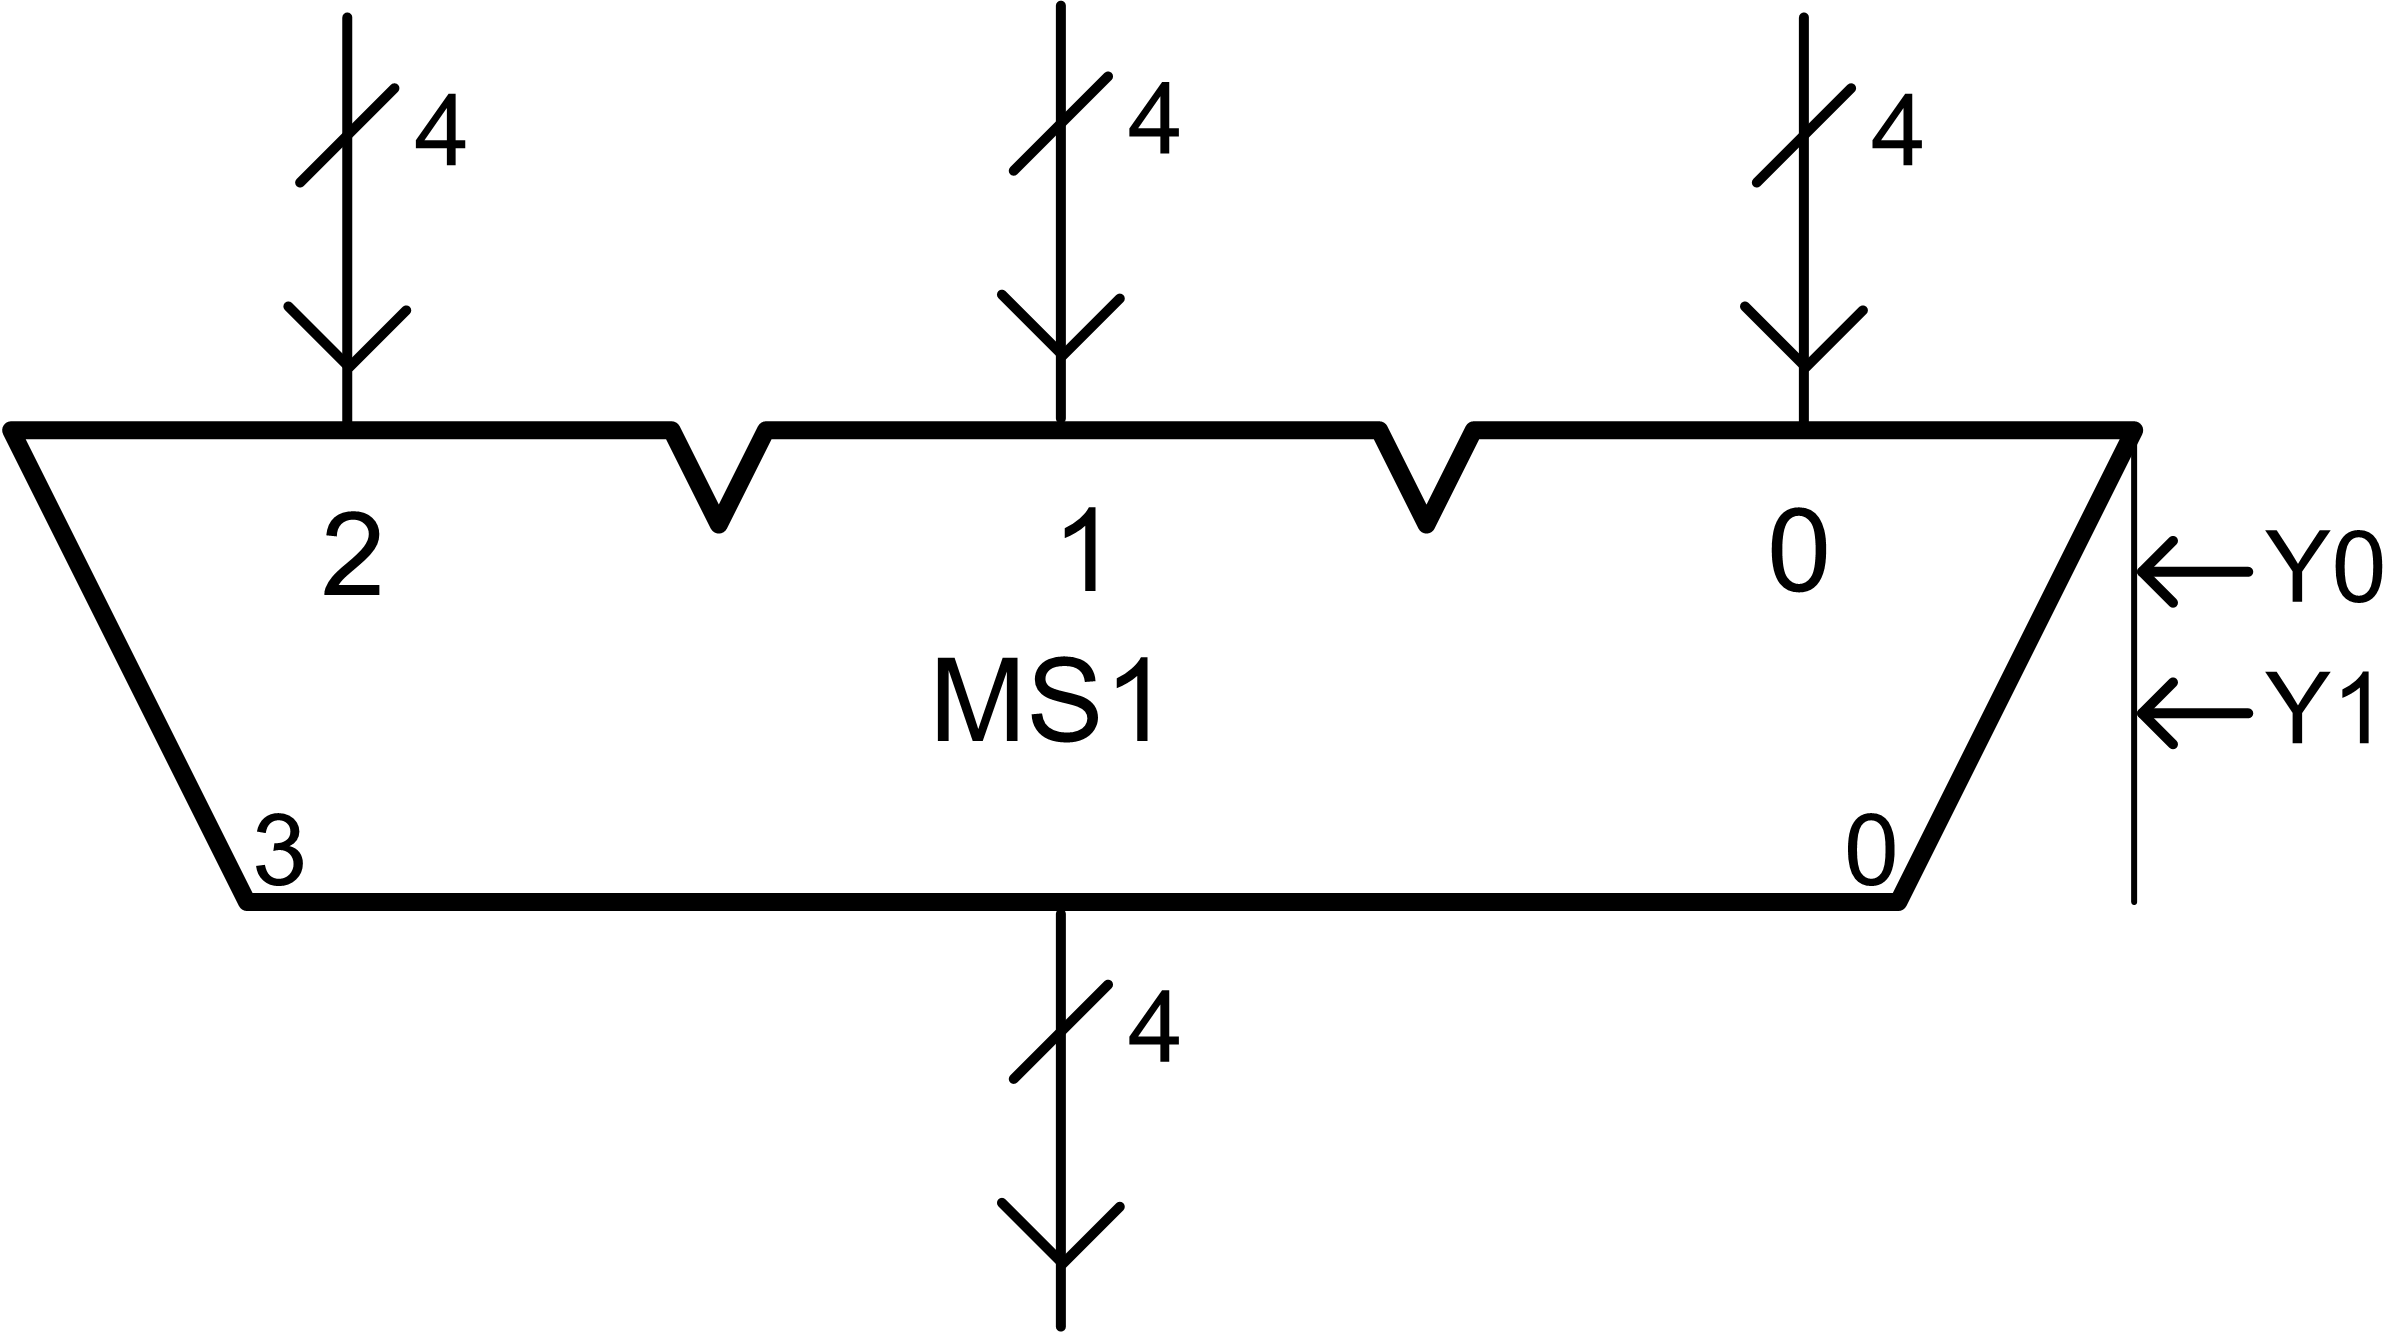
\includegraphics{fig/muxbig}
    \caption{Многоплечевой мультиплексор}
    \label{fig::ch::practice::muxbig}
\end{figure}


\subsubsection{Сумматор}

Условное графическое обозначение сумматора приведено на рисунке \ref{fig::ch::practice::summator}.
\begin{figure}[!ht]
    \centering
    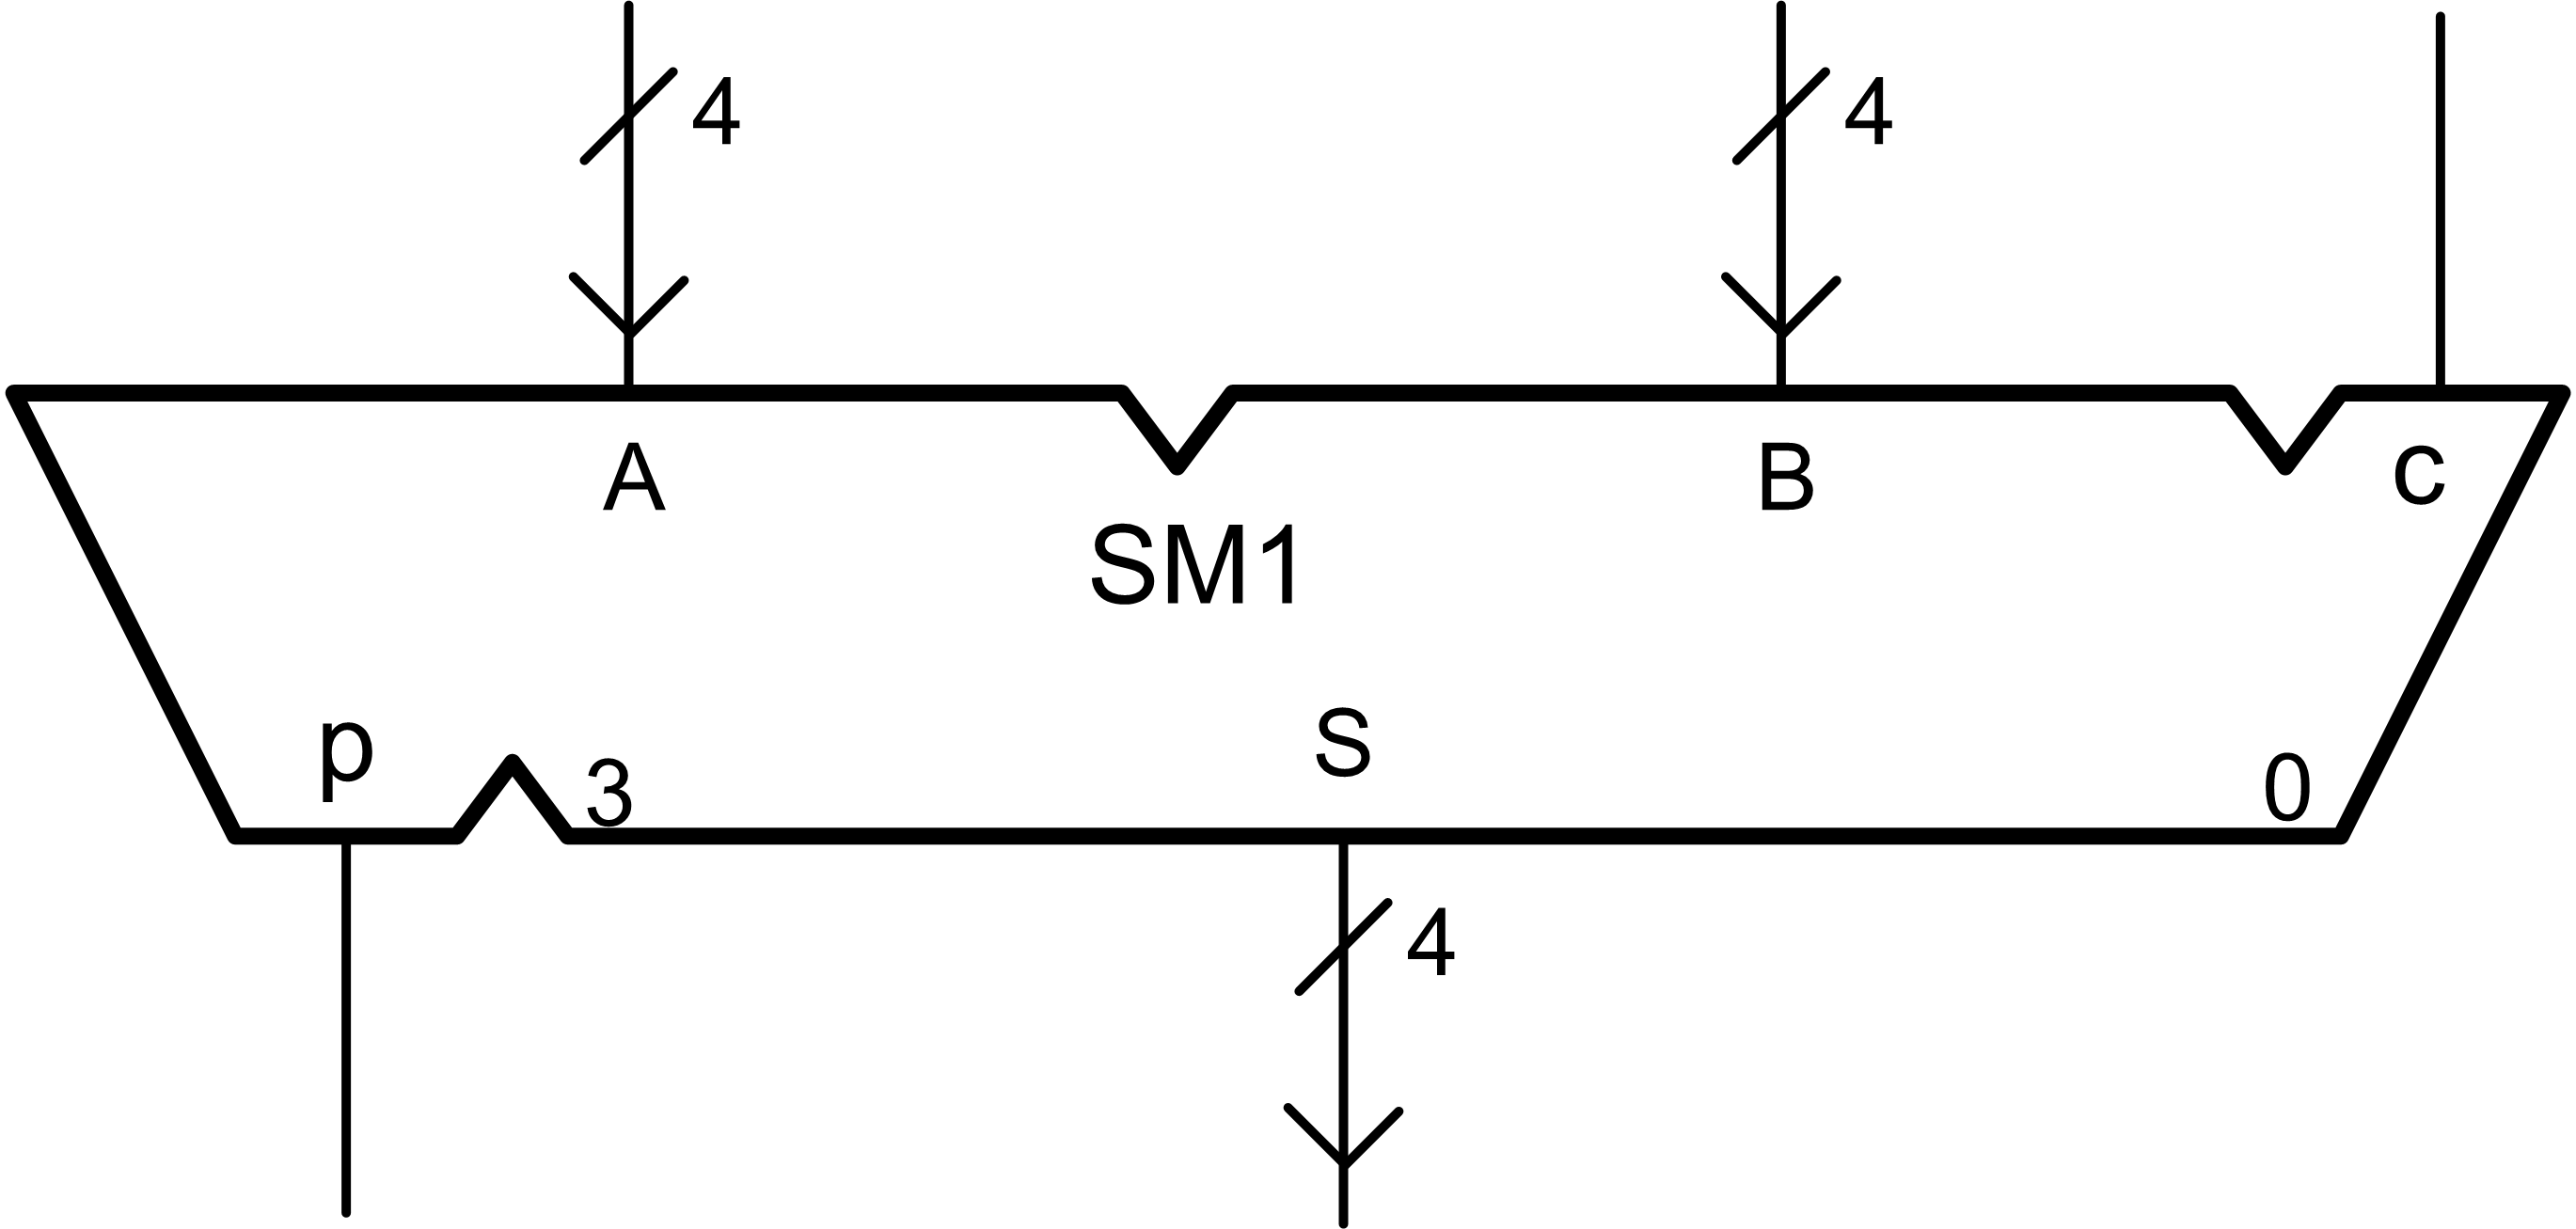
\includegraphics{fig/summator}
    \caption{Сумматор}
    \label{fig::ch::practice::summator}
\end{figure}

Сумматор выполняет арифметическое сложение $n$-разрядных входов (на рисунке \ref{fig::ch::practice::summator} $n=4$) входов $A$ и $B$ а также одноразрядного входа переноса в младшие разряды $c$. На выход $S$ выдаются младшие $n$ разрядов результата, а на выход $p$ --- бит переноса из старшего $(n-1)$-го разряда суммы $S$:
\begin{align*}
    S \equiv (A + B + c) \pmod{2^n};\\
    p = (A + B + c) \div{2^n}.
\end{align*}

В случае, если нужно получить сумматор большей разрядности на основе сумматоров меньшей разрядности, то выход переноса из старших разрядов младшего сумматора замыкают на вход переноса старшего сумматора (см. рисунок \ref{fig::ch::practice::summators}).
\begin{figure}[!ht]
    \centering
    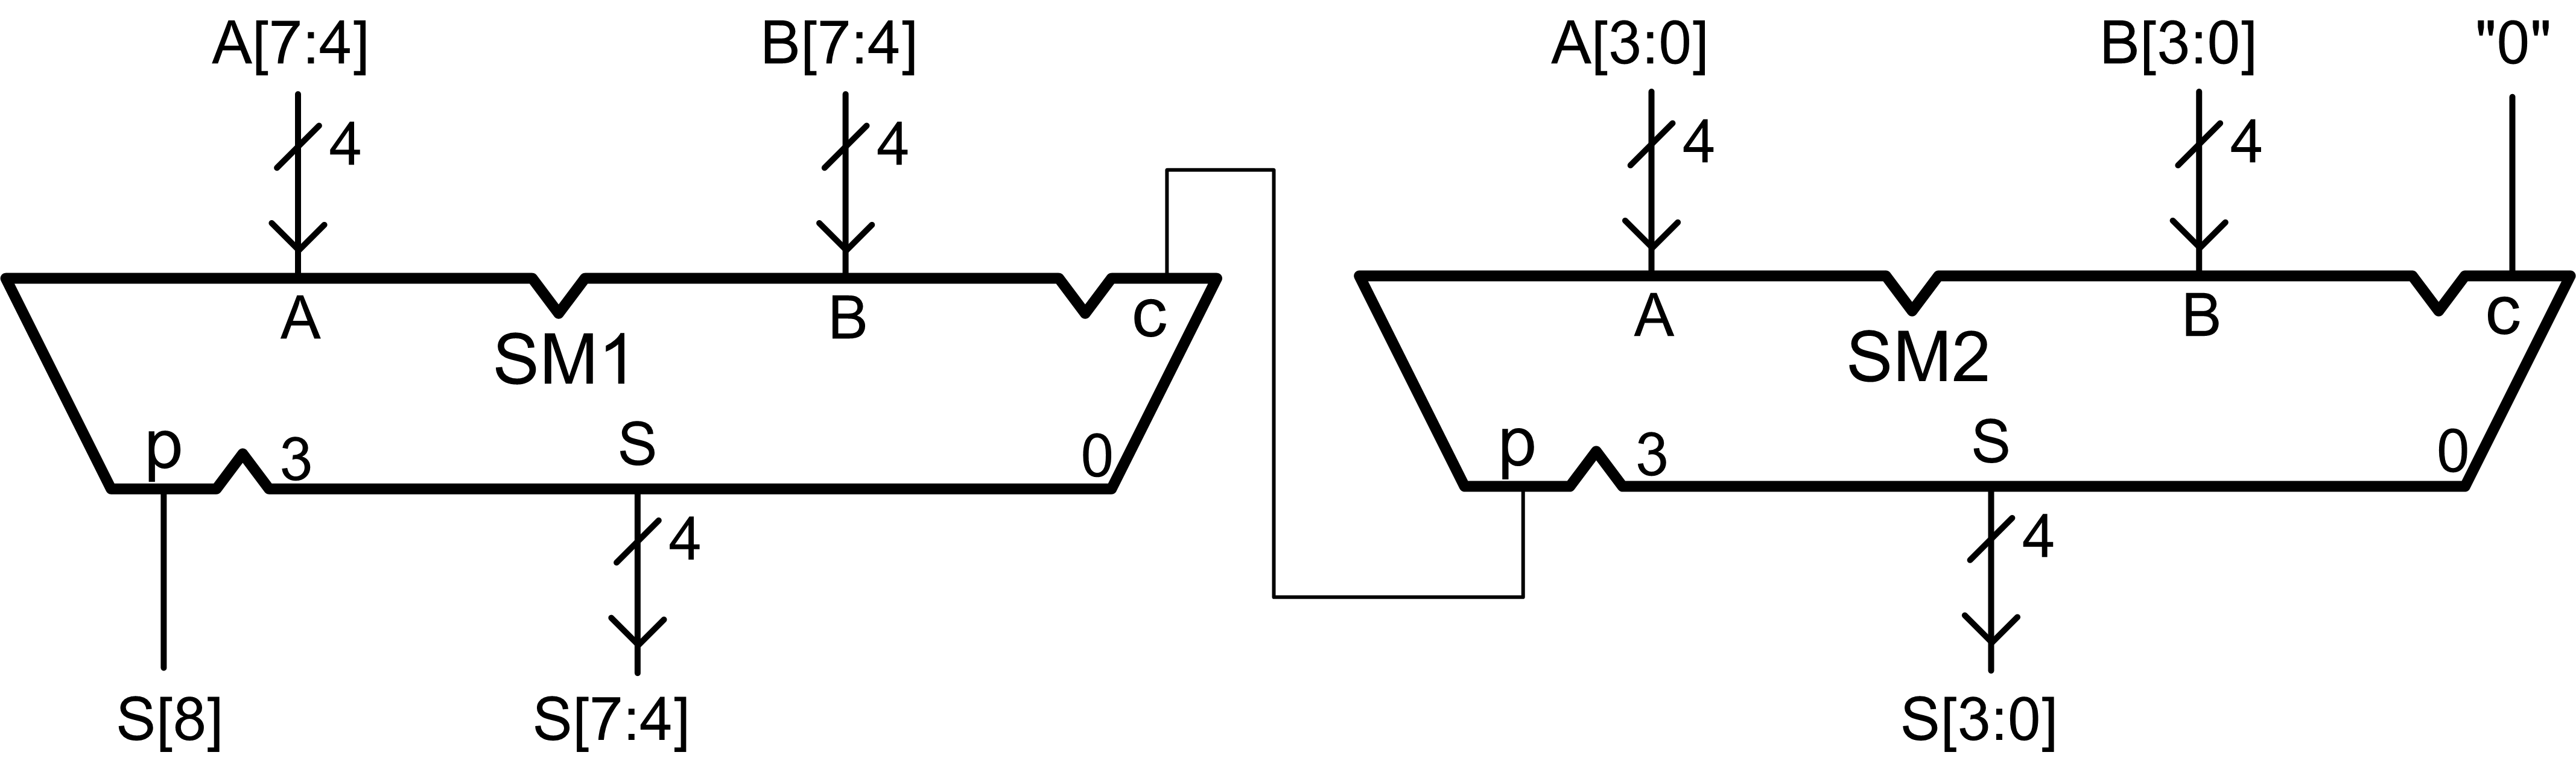
\includegraphics[width=.85\textwidth]{fig/summators}
    \caption{8-разрядный сумматор на основе двух 4-х разрядных}
    \label{fig::ch::practice::summators}
\end{figure}

На схемах сумматор любой разрядности рисуют одним элементом, если неважно, как этот сумматор устроен.


\subsubsection{Шинный формирователь}

Шинным формирователем устройство называется потому, что обычно его выходы подключены к шине. По управляюещму сигналу (на рисунке \ref{fig::ch::practice::zbuffer} сигнал $Y0$) шинный формирователь может отключать свои выходы от шины. Когда шинный формирователь подключен к шине, он выдает данные со входа на шину. Так как шина может быть общей для нескольких устройств, то использование шинных формирователей обязательно, чтобы гарантировать, что только одно устройство выдает на шину данные.

\begin{figure}[!ht]
    \centering
    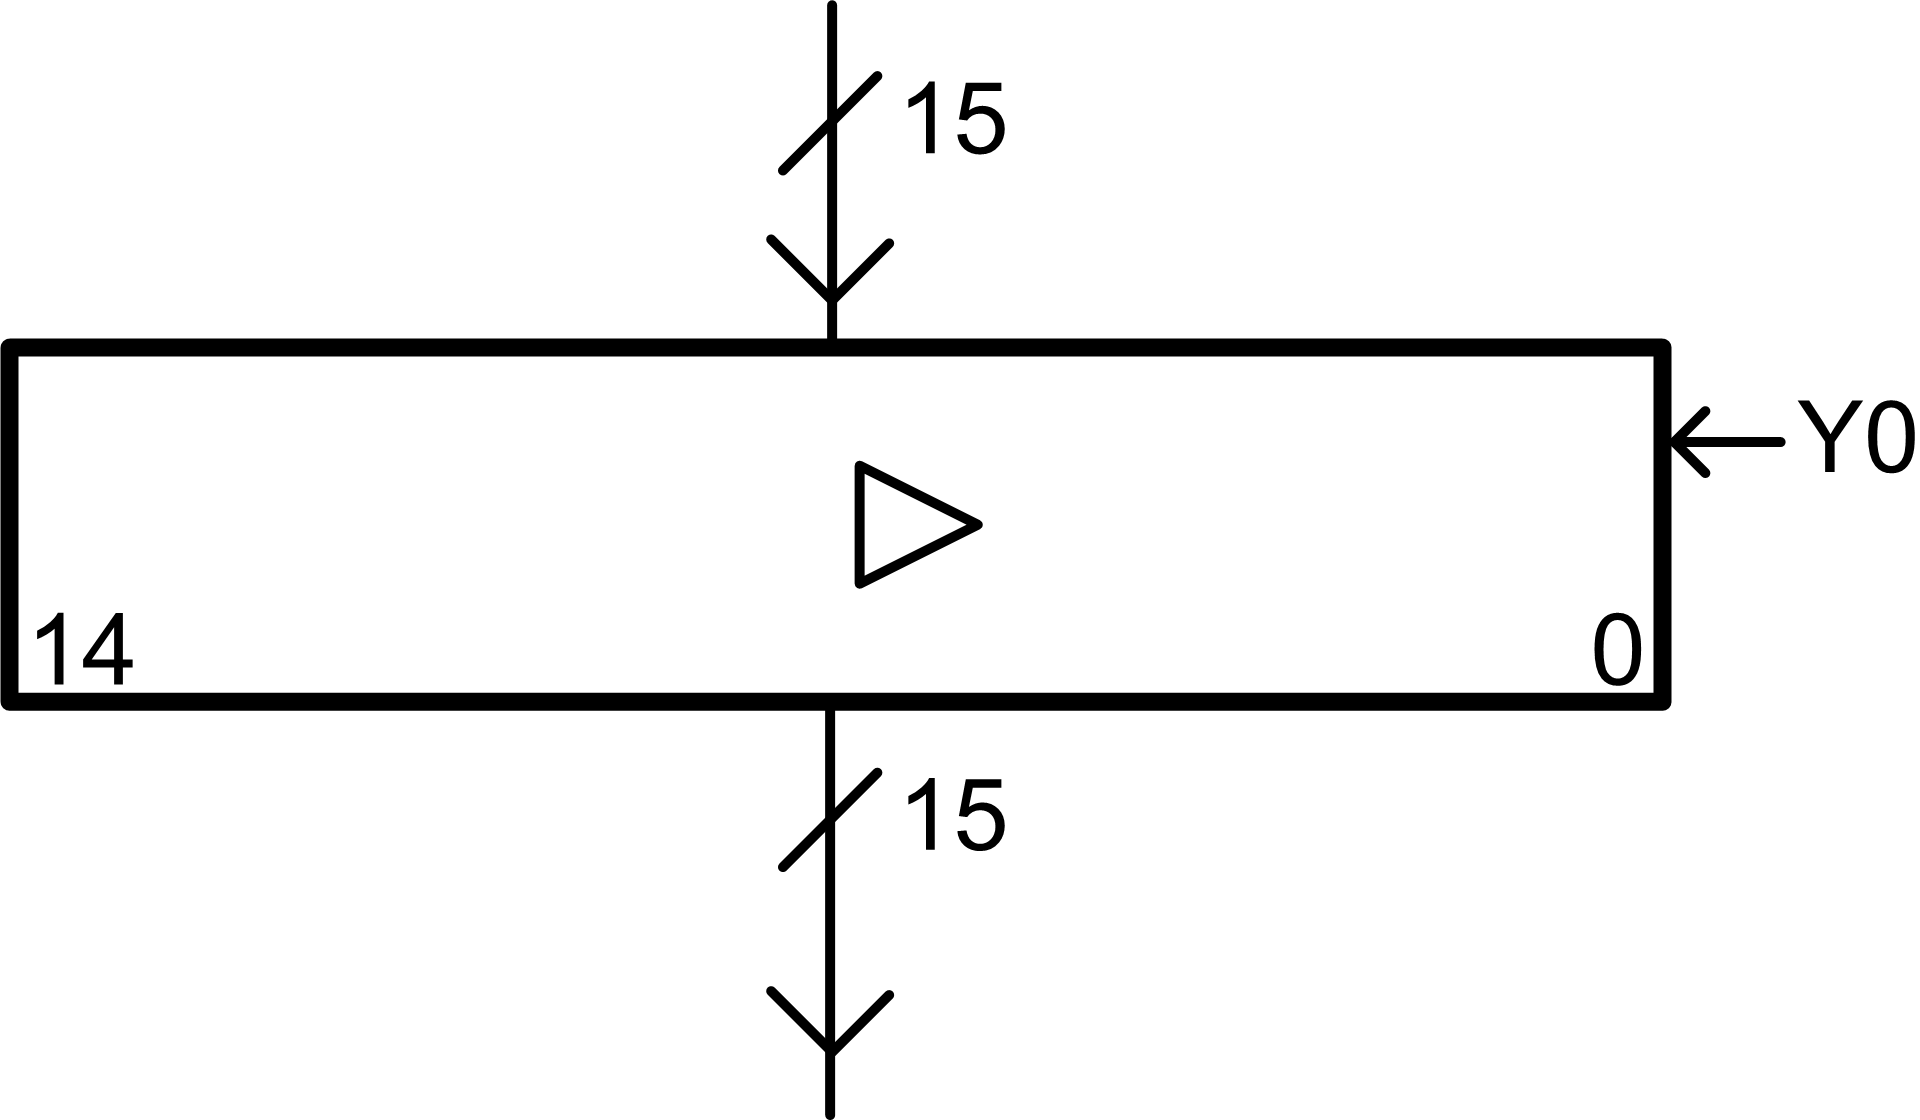
\includegraphics{fig/zbuffer}
    \caption{15-разрядный шинный формирователь}
    \label{fig::ch::practice::zbuffer}
\end{figure}


\subsection{Элементы памяти}

Элементы памяти могут сохрянять информацию (состояние) между тактами. Они обычно имеют управляющий сигнал, который управляет запоминанием информации со входов. Т.е. в течение такта такой элемент либо <<запоминает>> информацию со входов, либо хранит (или преобразует) ранее запомненную информацию.

\subsubsection{Регистры}
\label{sss::ch::practice::regiter}

Обычный регистр содержит автономную $n$-разрядную ячейку памяти и предназначен только для запоминания $n$ бит информации со входов. Помимо основной функции он может, например, выполнить сброс всех бит своей ячейки памяти в $0$ или $1$. На выходы регистра всегда выдается содержимое его внутренней ячейки памяти.

\begin{figure}[!ht]
    \centering
    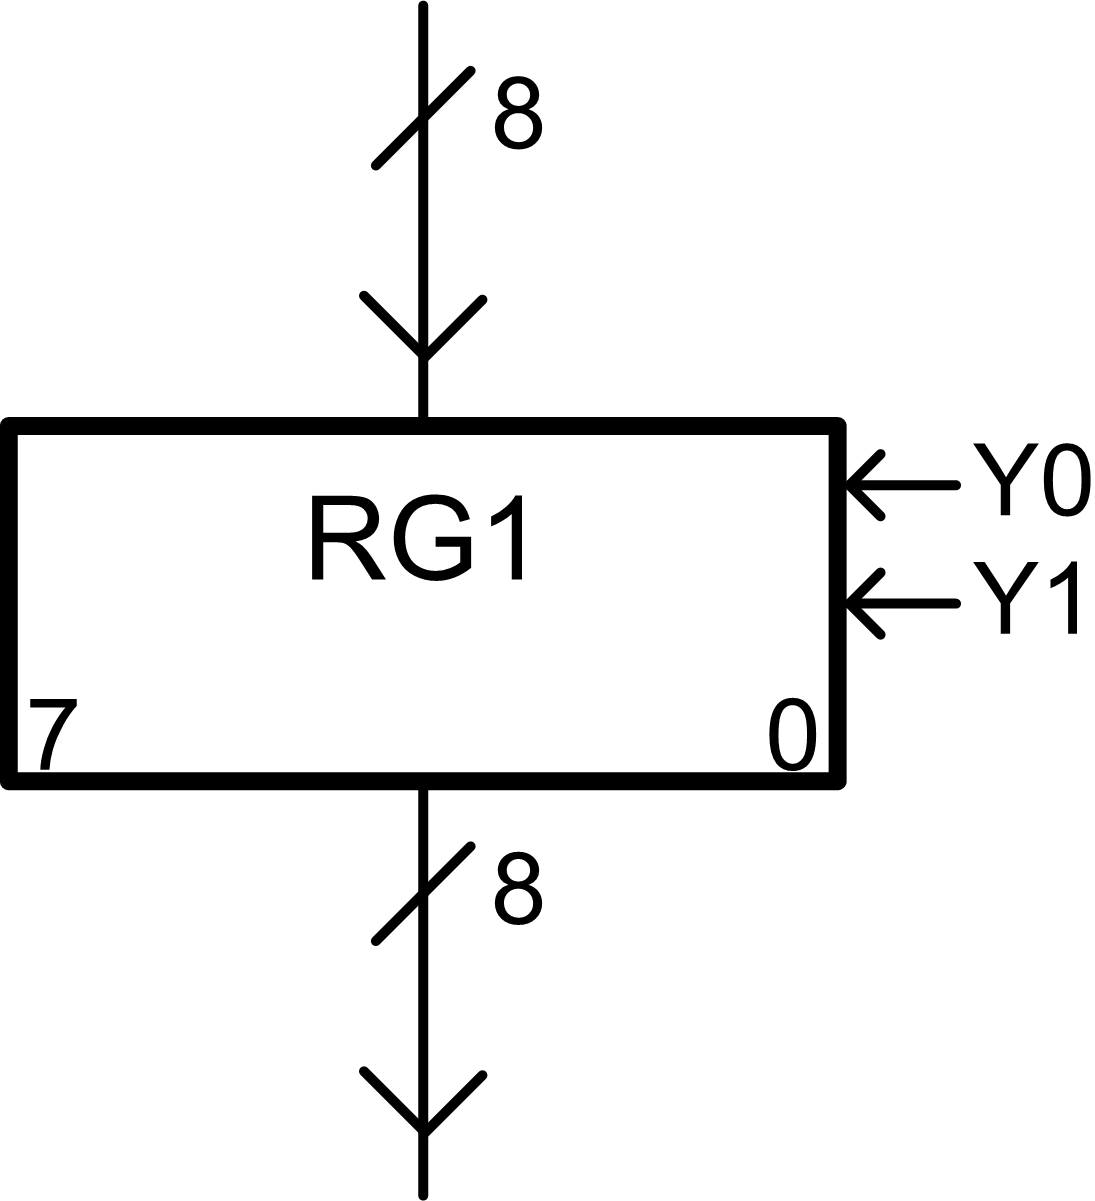
\includegraphics{fig/register}
    \caption{8-разрядный регистр}
    \label{fig::ch::practice::register}
\end{figure}

Например, на рисунке \ref{fig::ch::practice::register} изображен обычный регистр, расшифровка управляющих сигналов которого может быть следующей:
\begin{itemize}
    \item $Y0$ --- разрешение записи в $RG1$. Если данный сигнал подается в течение такта, то регистр <<запоминает>> информацию со входов и хранит до тех пор, пока $Y0$ вновь не будет подан в будущем.

    \item $Y1$ --- сброс всех разрядов внутренней ячейки памяти $RG1$ в $0$.
\end{itemize}

Управляющие сигналы регистра могут конфликтовать, например, состояние регистра не определено, если одновременно подать сигналы разрешения записи и сброса.

Сдвиговые регистры изображаются особым образом, в виде параллелограмма. Направление сдвига разрядов ячейки памяти обозначается стрелкой внутри регистра. Например, при сдвиге влево значение старшего разряда теряется, а в младший разряд заносится значение разряда со специального входа, который изображается боковой планкой с нужного края. 

\begin{figure}[!ht]
    \centering
    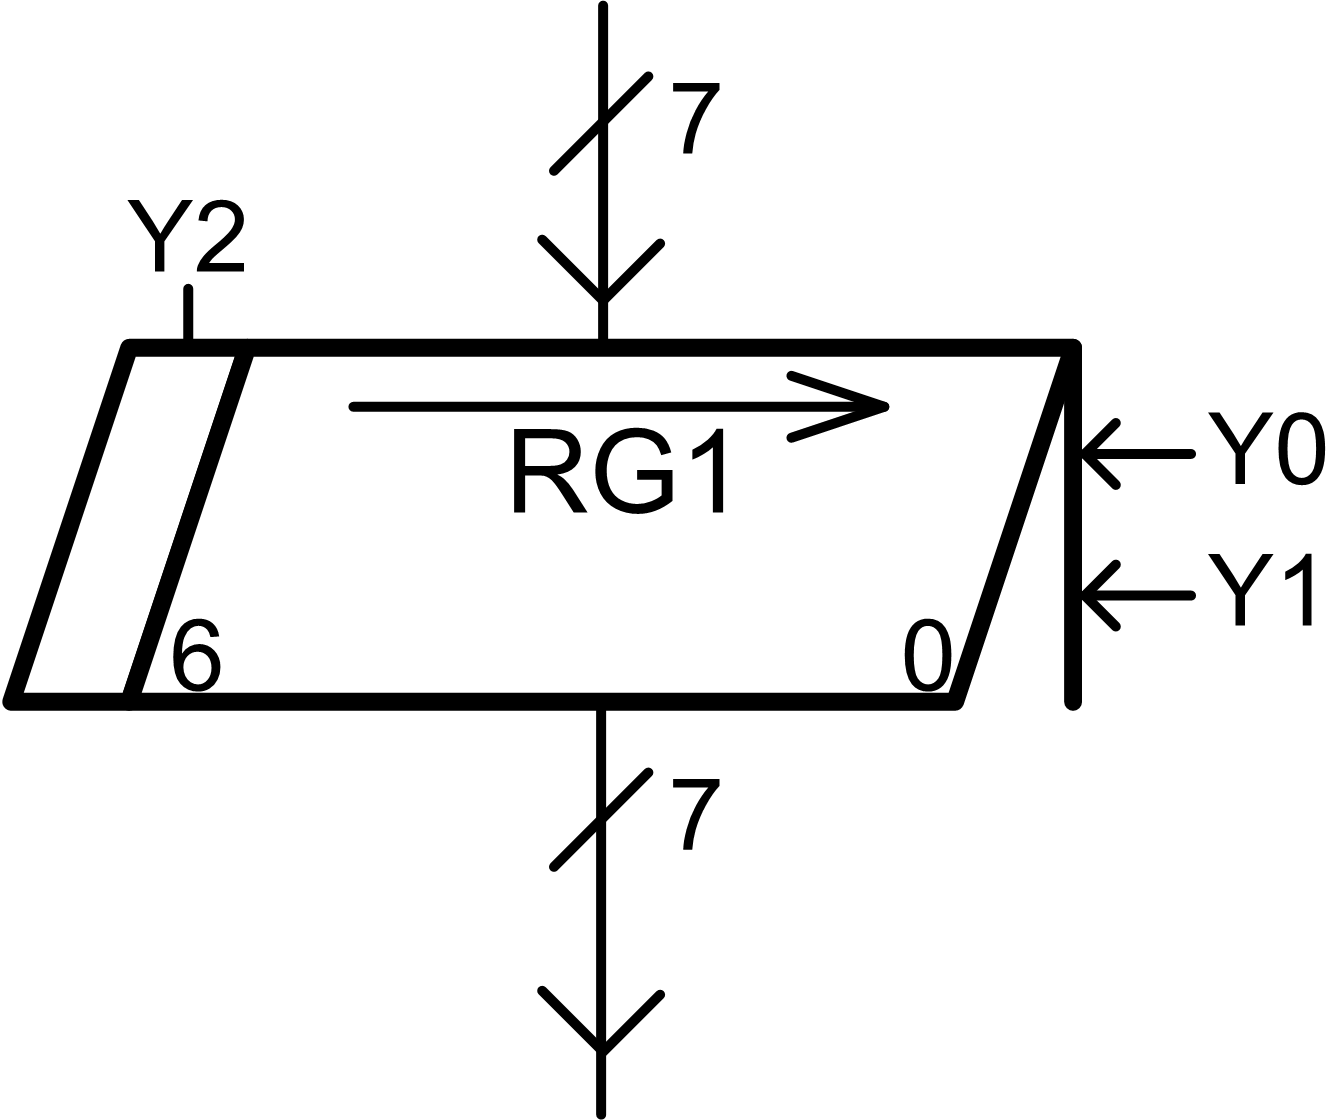
\includegraphics{fig/shiftregister}
    \caption{7-разрядный сдвиговый регистр}
    \label{fig::ch::practice::shiftregister}
\end{figure}

На рисунке \ref{fig::ch::practice::shiftregister} изображен сдвиговый регистр, расшифровка управляющих сигналов которого может быть следующей:
\begin{itemize}
    \item $Y0$ --- разрешение записи в $RG1$. Если данный сигнал подается в течение такта, то регистр <<запоминает>> информацию со входов и хранит до тех пор, пока $Y0$ вновь не будет подан в будущем.

    \item $Y1$ --- сдвиг $RG1$ вправо.
    
    \item вход $Y2$ определяет значение $6$-го разряда при сдвиге.
\end{itemize}


\subsubsection{Триггеры}

Триггер --- это одноразрядное запоминающее устройство. Триггеров существует несколько видов: D, RS, JK, \ldots В схемах будет использоваться D-триггер (см. рисунок \ref{fig::ch::practice::dtrigger}), который можно считать одноразрядным регистром: если на вход $C$ подается 1, то триггер <<запоминает>> бит информации со входа $D$, а если на вход $C$ подается 0, то триггер выдает ранее запомненный бит.

\begin{figure}[!ht]
    \centering
    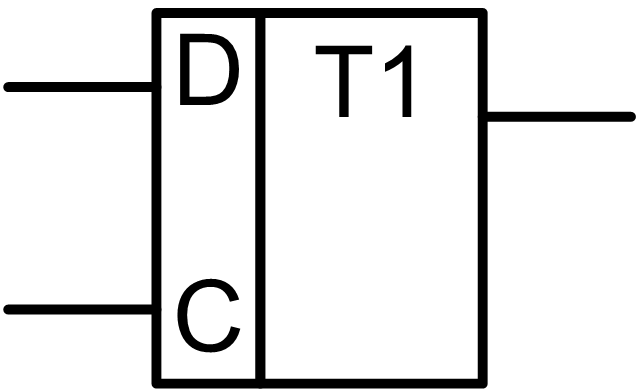
\includegraphics{fig/dtrigger}
    \caption{D-триггер}
    \label{fig::ch::practice::dtrigger}
\end{figure}
